\documentclass[12pt,a4paper]{article}
\usepackage[UTF8]{ctex}
\usepackage{amsmath,amssymb}
\usepackage{xcolor}
\usepackage{hyperref}
\usepackage{geometry}
\usepackage{graphicx}
\geometry{margin=2.5cm}

\title{Quantum Topological Data Analysis / 量子拓扑数据分析}
\author{QuoNic}
\date{}

\begin{document}
\maketitle

\begin{center}
\textbf{ML / 机器学习} | 难度：高级 | 预计时间：25 分钟
\end{center}

\tableofcontents
\newpage

\section{为什么需要？}

量子 TDA 是经典 TDA 的量子推广，用于分析数据的拓扑结构。

\subsection{经典局限}
\begin{itemize}
  \item 经典 TDA 计算持久同调慢
  \item 对于大规模数据，经典方法效率低
\end{itemize}

\subsection{量子优势}
\begin{itemize}
  \item 量子 TDA 可以在量子计算机上高效计算持久同调
  \item 提供指数加速
  \item 是量子拓扑学的基础
\end{itemize}

\subsection{实际应用}
\begin{itemize}
  \item 数据分析
  \item 机器学习
  \item 材料科学
\end{itemize}

\section{快速上手}

\begin{verbatim}
from quonic.ml import qtda

# 量子拓扑数据分析
data = [[0, 1], [1, 0], [1, 1], [0, 0]]
result = qtda(data)
print(f'Betti numbers: {result.betti}')
\end{verbatim}

\textbf{预期输出}：
\begin{verbatim}
Betti numbers: [1, 0]
\end{verbatim}

\section{原理详解}

\subsection{电路图}

\begin{center}
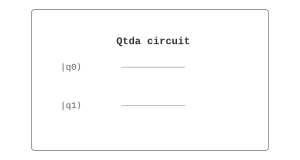
\includegraphics[width=0.6\textwidth]{../../images/qtda_circuit.svg}
\end{center}

\subsection{数学推导}

量子 TDA 基于量子相位估计：
\begin{equation}
|0\rangle|\psi\rangle \to |\tilde{\lambda}\rangle|\psi\rangle
\end{equation}

\textbf{持久同调}：
\begin{equation}
H_k(X_\epsilon) \to H_k(X_{\epsilon'})
\end{equation}

\subsection{几何解释}

量子 TDA 在量子态空间中分析数据的拓扑结构。量子相位估计可以高效计算持久同调。

\section{代码详解}

\begin{verbatim}
from quonic.ml import qtda

# qtda(data, max_dimension)
# data: 输入数据
# max_dimension: 最大维度
result = qtda(data, max_dimension=2)

# result.betti: Betti 数
# result.persistence: 持久图
print(f'Betti numbers: {result.betti}')
\end{verbatim}

\section{进阶用法}

\subsection{场景 1：点云数据}

\begin{verbatim}
from quonic.ml import qtda

# 点云数据的拓扑分析
points = generate_pointsphere(n_points=100)
result = qtda(points)
print(f'Betti numbers: {result.betti}')
\end{verbatim}

\section{适用场景}

\subsection{数据分析}

量子 TDA 可以分析数据的拓扑结构，如孔洞、连通分量等。传统 TDA 计算慢，量子 TDA 可以提供指数加速。

\subsection{材料科学}

量子 TDA 可以分析材料的微观结构。例如，分析多孔材料的孔洞结构、分析晶体的缺陷等。

\section{常见问题}

\subsection{量子 TDA 和经典 TDA 有什么区别？}

量子 TDA 使用量子相位估计计算持久同调，可以在 $O(\log N)$ 时间内完成，经典 TDA 需要 $O(N^3)$ 时间。

\subsection{量子 TDA 的精度如何？}

精度取决于量子相位估计的精度。

\section{学习路径}

\subsection{前置知识}
\begin{itemize}
  \item 拓扑数据分析
  \item 量子相位估计
  \item 持久同调
\end{itemize}

\subsection{继续学习}
\begin{itemize}
  \item 量子机器学习
  \item 量子拓扑学
  \item 材料科学
\end{itemize}

\section{完整示例代码}

\subsection{示例 1：基本量子 TDA}

\begin{verbatim}
from quonic.ml import qtda

data = [[0, 1], [1, 0], [1, 1], [0, 0]]
result = qtda(data)
print(f'Betti numbers: {result.betti}')
\end{verbatim}

\section{下载}

\begin{itemize}
  \item [qtda.py](https://github.com/ChrisLee0721/QuoNic/blob/main/examples/qtda/qtda.py)
\end{itemize}

\end{document}
